\documentclass[10pt]{beamer}

\usetheme{metropolis}

\title{Introduction to Machine Learning}

\begin{document}

\maketitle

\begin{frame}{Concept}

The course is organized as a digital lecture, which should be as self-contained and enable self-study as much as possible:

  \begin{itemize}
    \item
      Slides with lecture videos

    \item
      Interactive tutorials

    \item
       Complemented by a week-long inverted-classroom block course

  \end{itemize}

\end{frame}

\begin{frame}{Concept - Lecture Videos}

  \begin{center}
  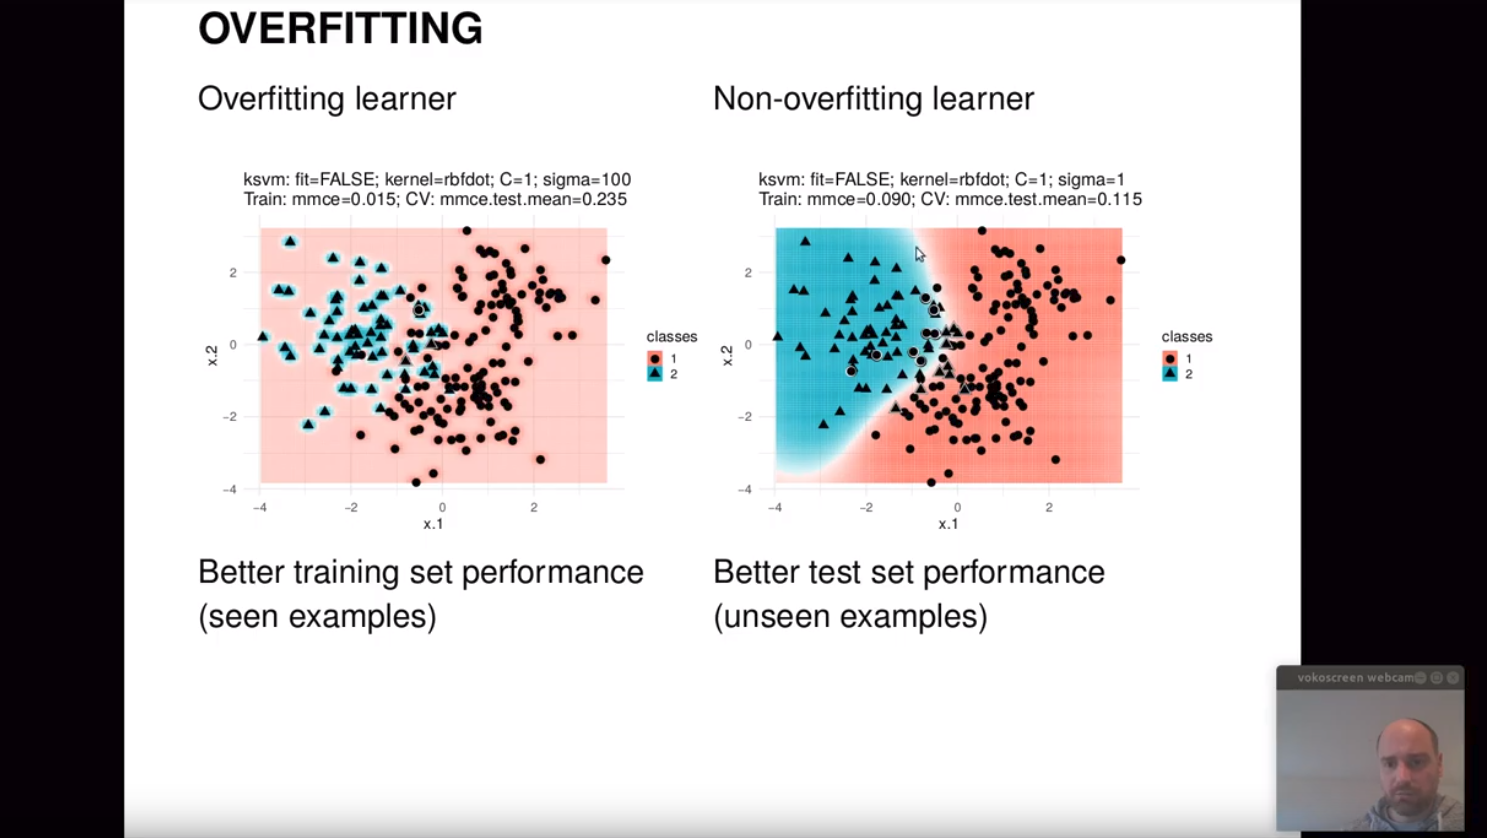
\includegraphics[width=\textwidth]{iml_video.png}
  \end{center}

\end{frame}

\begin{frame}{Concept - Interactive Tutorials (Quiz)}

  \begin{center}
  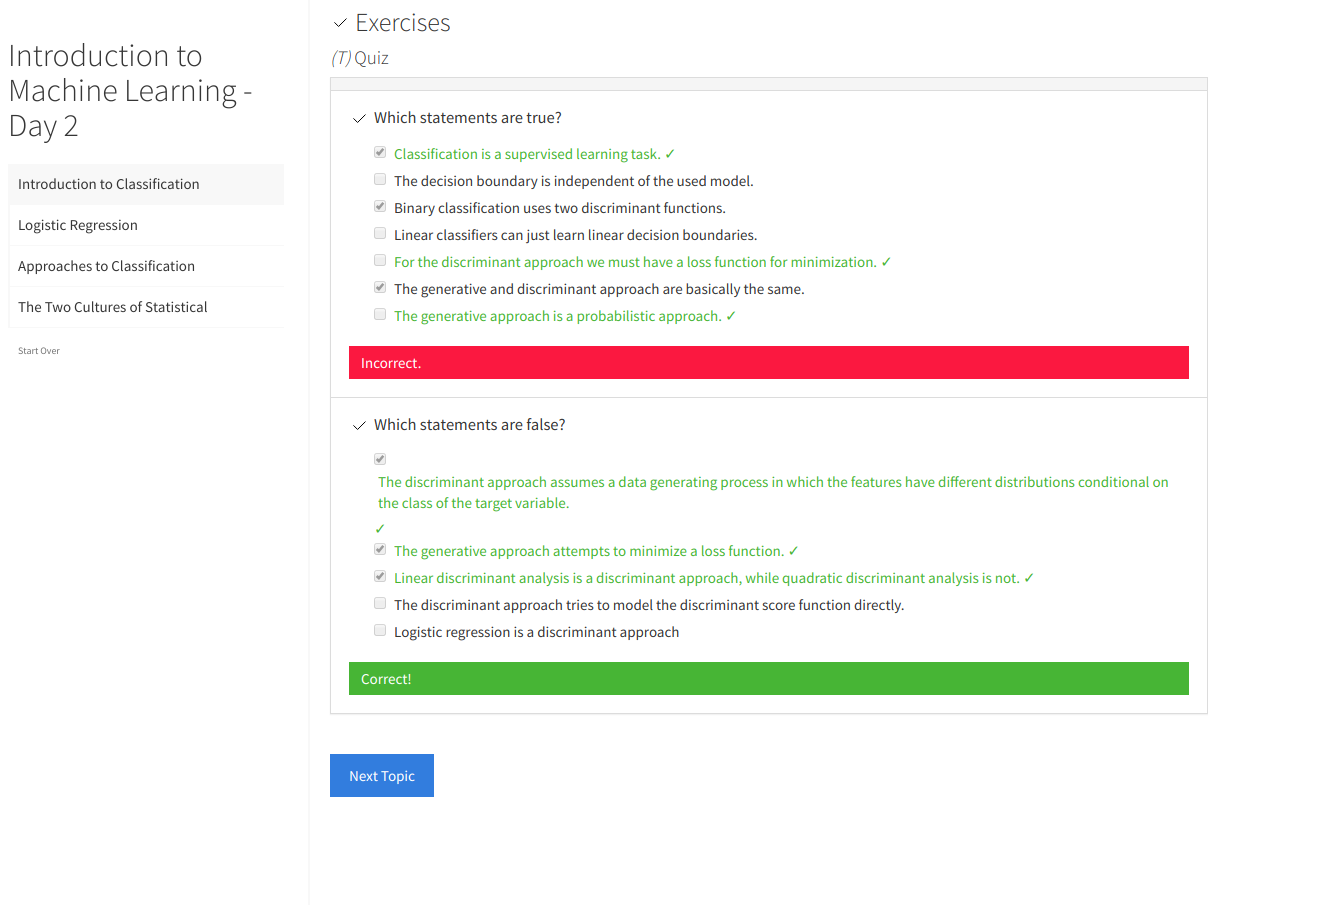
\includegraphics[width=\textwidth]{iml_tut0.png}
  \end{center}

\end{frame}

\begin{frame}{Concept - Interactive Tutorials (Examples)}

  \begin{center}
  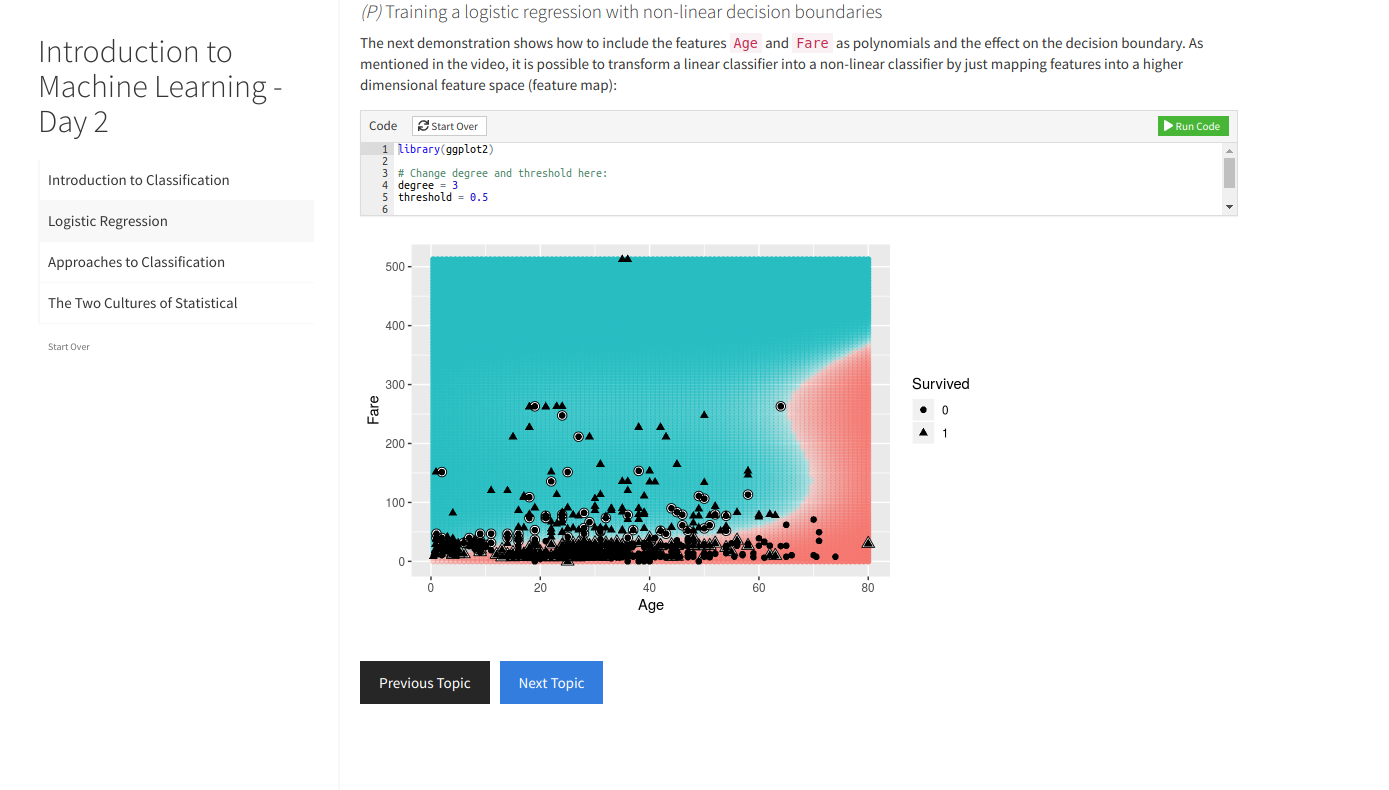
\includegraphics[width=\textwidth]{iml_tut1.png}
  \end{center}

\end{frame}

\end{document}
